\documentclass[a4paper]{article}
\usepackage[utf8]{inputenc}
\usepackage{geometry}
\usepackage{graphicx}
\usepackage{subfigure}
\geometry{a4paper,scale=0.85}

\title{Fast Solvers for Large Systems of Equations}
\author{Shuai Lu 170742}
\date{Homework 2}

\begin{document}
\maketitle
\noindent \textbf{Exercise 2.1*} (a) [1 point] Consider a linear system $\mathbf{A u}=\mathbf{f}$ (with a nonsingular matrix $\mathbf{A}$ ) and a linear iterative method
$$
\mathbf{u}^{(k+1)}=\mathbf{M u}^{(k)}+\mathbf{N f}
$$
for its solution. Show that if the exact solution $\mathbf{u}^{*}$ of the system for an arbitrary $\mathbf{f}$ is a fixed point of this method, this recurrence can be represented in form
$$
\mathbf{u}^{(k+1)}=\mathbf{u}^{(k)}+\mathbf{N}\left(\mathbf{f}-\mathbf{A} \mathbf{u}^{(k)}\right)
$$
Why only non-singular $\mathbf{N}$ make sense in these methods, so that we can set $\mathbf{N}=\mathbf{W}^{-1}$ for some $\mathbf{W} ?$ Which $\mathbf{W}$ would be theoretically the best choice (so that the method solves the system in one iteration)?\\

\noindent Solution:\\
Since the $\mathbf{u}^{*}$ is the fixed point of this method, we can get\\
$$
\left( \mathbf{I}-\mathbf{M} \right) \mathbf{u}^{\left( * \right)}=\mathbf{Nf}=\mathbf{NAu}^{\left( * \right)}
\\
\Rightarrow \mathbf{Mu}^{\left( * \right)}=\left( \mathbf{I}-\mathbf{NA} \right) \mathbf{u}^{\left( * \right)}
$$
Replace the $\mathbf{Mu}^{\left( k \right)}$ with $\left( \mathbf{I}-\mathbf{NA} \right) \mathbf{u}^{\left( k \right)}$, so we can get\\
$$
\mathbf{u}^{\left( k+1 \right)}=\left( \mathbf{I}-\mathbf{NA} \right) \mathbf{u}^{\left( k \right)}+\mathbf{Nf}=\mathbf{u}^{\left( k \right)}+\mathbf{N}\left( \mathbf{f}-\mathbf{Au}^{\left( k \right)} \right) 
$$
Why only non-singular?\\
The linear system can be solved in one iteration\\
$$
\mathbf{u}^{\left( * \right)}=\mathbf{u}^{\left( 0 \right)}+\mathbf{N}\left( \mathbf{f}-\mathbf{Au}^{\left( 0 \right)} \right) 
\\
\Rightarrow \mathbf{Au}^{\left( * \right)}=\mathbf{Au}^{\left( 0 \right)}+\mathbf{AN}\left( \mathbf{f}-\mathbf{Au}^{\left( 0 \right)} \right) =\mathbf{f}
\\
\Rightarrow \mathbf{A}\left( \mathbf{I}-\mathbf{NA} \right) \mathbf{u}^{\left( 0 \right)}=\left( \mathbf{I}-\mathbf{AN} \right) \mathbf{f}
$$
So $\mathbf{NA}=\mathbf{I}, \mathbf{W}=\mathbf{A}$.\\

\noindent (b) $\left[1\right.$ point] Let $\mathbf{e}^{(k)}:=\mathbf{u}^{(k)}-\mathbf{u}^{*}$ be the error. How does this error relate to the residual $\mathbf{r}^{(k)}:=\mathbf{f}-\mathbf{A u}^{(k)} ?$ (Write the function $\mathbf{r}(\mathbf{e})$ that maps the error to the residual.) For a vector norm $\|\cdot\|$, is $\|\mathbf{r}(\mathbf{e})\|$ a norm of the error? Write a formula for the dependence of $\mathbf{e}^{(k+1)}$ on $\mathbf{e}^{(k)}$.\\

\noindent Solution:\\
\noindent $$
\mathbf{r}^{\left( k \right)}:=\mathbf{f}-\mathbf{Au}^{\left( k \right)}=\mathbf{A}\left( \mathbf{u}^{\left( * \right)}-\mathbf{u}^{\left( k \right)} \right) =-\mathbf{Ae}^{\left( k \right)}
$$
\\
Since $\| \mathbf{r}\left( \mathbf{e} \right) \| =\| \mathbf{Ae} \|\ge 0$, it satisfied Semi positivity, Linearity, Triangle inequality. Because $\mathbf{A}$ is non-singular, $\| \mathbf{Ae} \|= 0$ iff $\mathbf{e}= 0$.\\

\noindent (c) [1 point] Write the $\mathbf{W}$ matrix of the Gauss-Seidel method in the lexicographical ordering.\\

\noindent Solution:\\

\noindent $A_{11},0,A_{21},A_{22}$.\\

\noindent \textbf{Exercise 2.2*} (a) [2 points] How many arithmetical operations is necessary to solve a linear system $\mathbf{A u}=\mathbf{f}$ with a (dense) $n \times n$-matrix $\mathbf{A}$ using the Gaussian elimination? Represent the result in the form $O\left(n^{\alpha}\right)$ for some $\alpha$.\\

\noindent Solution:\\

\noindent When using the first row to eliminate the first elements in other rows, we need $ n\times \left( n-1 \right) $
operations. We need to redo for second row, until last row. So the total operations are $ O\left( n^3 \right) $.\\

\noindent (b) [2points] A sparse matrix can be represented by a graph with the points associated (in particular, geometrically) with the degrees of freedom. The edges (the arrows) denote the non-zero coefficients. Consider the cartesian grid on a unit square with $h=\frac{1}{4}$ (i.e. $N=4$ ) and the 5 -point stencil from Ex. $1.3$ on it. Plot the graph of the matrix defined by the 5 -point stencil. (Consider only the inner grid points.) Perform the Gaussian elimination. How is the graph of the matrix changed at every step of the elimination? (Plot the graphs.)\\

\noindent Solution:\\
\begin{figure}[htbp]
	\centering
	\begin{minipage}[t]{0.7\textwidth}
		\centering		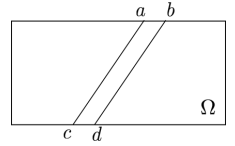
\includegraphics[width=10cm]{1.png}
	\end{minipage}
\end{figure}
\begin{figure}[htbp]
	\centering
	\begin{minipage}[t]{0.7\textwidth}
		\centering		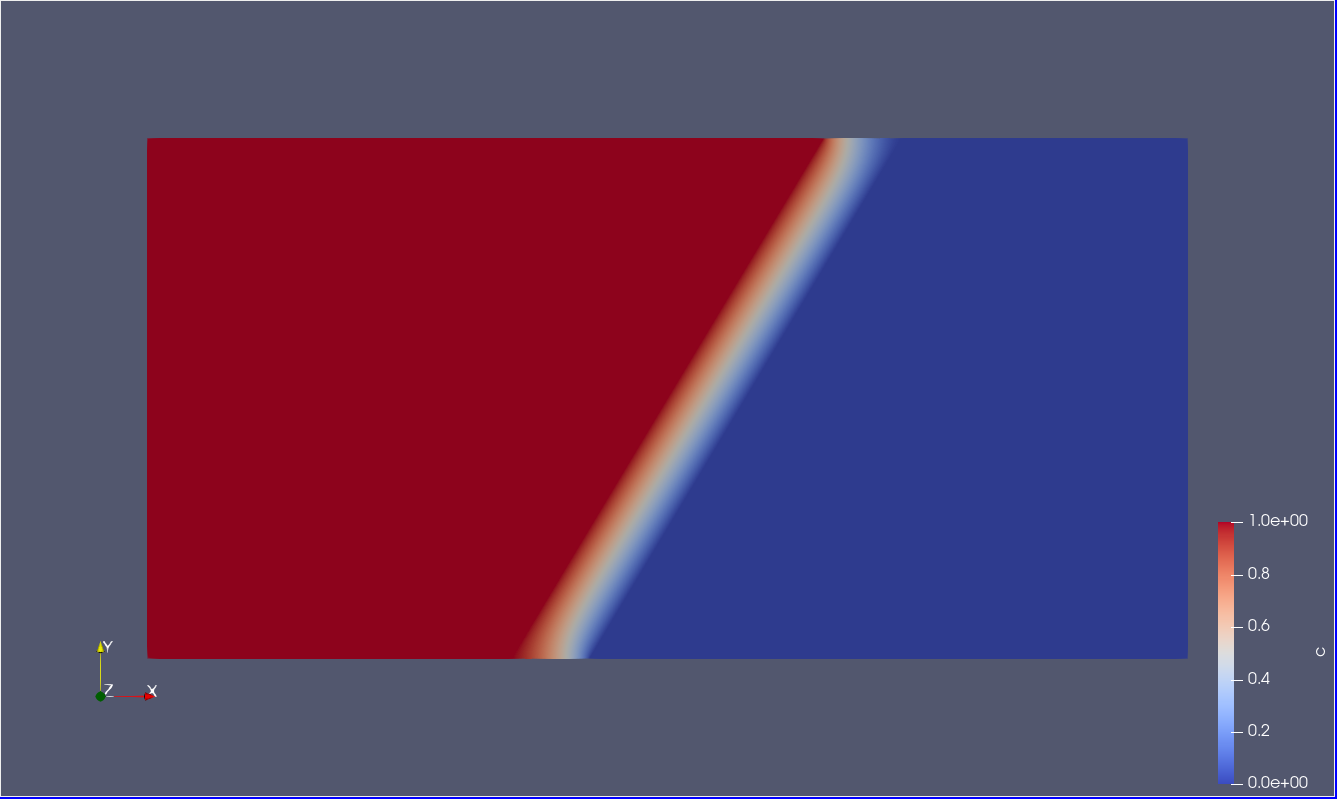
\includegraphics[width=10cm]{2.png}
	\end{minipage}
\end{figure}
\begin{figure}[htbp]
	\centering
	\begin{minipage}[t]{0.7\textwidth}
		\centering		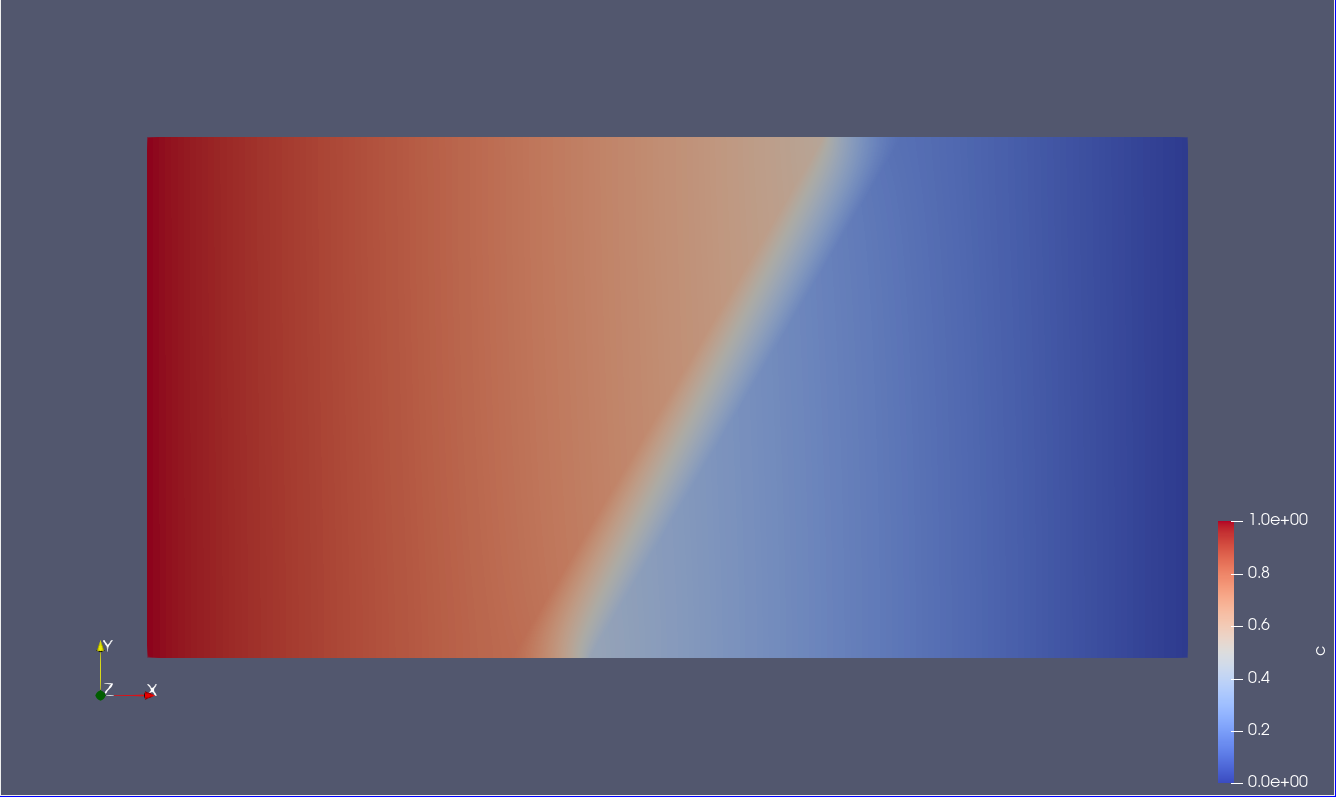
\includegraphics[width=10cm]{3.png}
	\end{minipage}
\end{figure}

\noindent (c) [1 points] During the Gaussian elimination in this matrix, only the band between the outer diagonals is filled with non-zeros. If we avoid operations beyond this band, what is the computational complexity of this method (in form of $O\left(N^{\beta}\right)$\\

\noindent Solution:\\

\noindent When using the first row to eliminate the first elements in other rows, we need $ C \left( n-1 \right) $
operations. We need to redo for second row, until last row. So the total operations are $ O\left( n^2 \right) $.\\

\noindent (d) [2 points] The idea of the ILU method is to neglect the newly arising edges. Compute the U matrix of the ILU method.\\

\noindent Solution:\\

$$
\left[\begin{array}{lllllllll}
	4 & -1 & 0 & -1 & 0 & 0 & 0 & 0 & 0 \\
	-1 & 4 & -1 & 0 & -1 & 0 & 0 & 0 & 0 \\
	0 & -1 & 4 & 0 & 0 & -1 & 0 & 0 & 0 \\
	-1 & 0 & 0 & 4 & -1 & 0 & -1 & 0 & 0 \\
	0 & -1 & 0 & -1 & 4 & -1 & 0 & -1 & 0 \\
	0 & 0 & -1 & 0 & -1 & 4 & 0 & 0 & -1 \\
	0 & 0 & 0 & -1 & 0 & 0 & 4 & -1 & 0 \\
	0 & 0 & 0 & 0 & -1 & 0 & -1 & 4 & -1 \\
	0 & 0 & 0 & 0 & 0 & -1 & 0 & -1 & 4
\end{array}\right] \rightarrow\left[\begin{array}{ccccccccc}
	1 & -\frac{1}{4} & 0 & -\frac{1}{4} & 0 & 0 & 0 & 0 & 0 \\
	0 & \frac{15}{4} & -1 & 0 & -1 & 0 & 0 & 0 & 0 \\
	0 & -1 & 4 & 0 & 0 & -1 & 0 & 0 & 0 \\
	0 & 0 & 0 & \frac{15}{4} & -1 & 0 & -1 & 0 & 0 \\
	0 & -1 & 0 & -1 & 4 & -1 & 0 & -1 & 0 \\
	0 & 0 & -1 & 0 & -1 & 4 & 0 & 0 & -1 \\
	0 & 0 & 0 & -1 & 0 & 0 & 4 & -1 & 0 \\
	0 & 0 & 0 & 0 & -1 & 0 & -1 & 4 & -1 \\
	0 & 0 & 0 & 0 & 0 & -1 & 0 & -1 & 4
\end{array}\right]
$$
$$
\rightarrow\left[\begin{array}{ccccccccc}
	1 & -\frac{1}{4} & 0 & -\frac{1}{4} & 0 & 0 & 0 & 0 & 0 \\
	0 & 1 & -\frac{4}{15} & 0 & -\frac{4}{15} & 0 & 0 & 0 & 0 \\
	0 & 0 & \frac{56}{15} & 0 & 0 & -1 & 0 & 0 & 0 \\
	0 & 0 & 0 & \frac{15}{4} & -1 & 0 & -1 & 0 & 0 \\
	0 & 0 & 0 & -1 & \frac{56}{15} & -1 & 0 & -1 & 0 \\
	0 & 0 & -1 & 0 & -1 & 4 & 0 & 0 & -1 \\
	0 & 0 & 0 & -1 & 0 & 0 & 4 & -1 & 0 \\
	0 & 0 & 0 & 0 & -1 & 0 & -1 & 4 & -1 \\
	0 & 0 & 0 & 0 & 0 & -1 & 0 & -1 & 4
\end{array}\right] \rightarrow\left[\begin{array}{ccccccccc}
	1 & -\frac{1}{4} & 0 & -\frac{1}{4} & 0 & 0 & 0 & 0 & 0 \\
	0 & 1 & -\frac{4}{15} & 0 & -\frac{4}{15} & 0 & 0 & 0 & 0 \\
	0 & 0 & 1 & 0 & 0 & -\frac{15}{56} & 0 & 0 & 0 \\
	0 & 0 & 0 & \frac{15}{4} & -1 & 0 & -1 & 0 & 0 \\
	0 & 0 & 0 & -1 & \frac{56}{15} & -1 & 0 & -1 & 0 \\
	0 & 0 & 0 & 0 & -1 & \frac{209}{56} & 0 & 0 & -1 \\
	0 & 0 & 0 & -1 & 0 & 0 & 4 & -1 & 0 \\
	0 & 0 & 0 & 0 & -1 & 0 & -1 & 4 & -1 \\
	0 & 0 & 0 & 0 & 0 & -1 & 0 & -1 & 4
\end{array}\right]
$$
$$
\rightarrow\left[\begin{array}{ccccccccc}
	1 & -\frac{1}{4} & 0 & -\frac{1}{4} & 0 & 0 & 0 & 0 & 0 \\
	0 & 1 & -\frac{4}{15} & 0 & -\frac{4}{15} & 0 & 0 & 0 & 0 \\
	0 & 0 & 1 & 0 & 0 & -\frac{15}{56} & 0 & 0 & 0 \\
	0 & 0 & 0 & 1 & -\frac{4}{15} & 0 & -\frac{4}{15} & 0 & 0 \\
	0 & 0 & 0 & 0 & \frac{52}{15} & -1 & 0 & -1 & 0 \\
	0 & 0 & 0 & 0 & -1 & \frac{209}{56} & 0 & 0 & -1 \\
	0 & 0 & 0 & 0 & 0 & 0 & \frac{56}{15} & -1 & 0 \\
	0 & 0 & 0 & 0 & -1 & 0 & -1 & 4 & -1 \\
	0 & 0 & 0 & 0 & 0 & -1 & 0 & -1 & 4
\end{array}\right] \rightarrow\left[\begin{array}{ccccccccc}
	-\frac{1}{4} & 0 & -\frac{1}{4} & 0 & 0 & 0 & 0 & 0 \\
	0 & 1 & -\frac{4}{15} & 0 & -\frac{4}{15} & 0 & 0 & 0 & 0 \\
	0 & 0 & 1 & 0 & 0 & -\frac{15}{56} & 0 & 0 & 0 \\
	0 & 0 & 0 & 1 & -\frac{4}{15} & 0 & -\frac{4}{15} & 0 & 0 \\
	0 & 0 & 0 & 0 & 1 & -\frac{15}{52} & 0 & -\frac{15}{52} & 0 \\
	0 & 0 & 0 & 0 & 0 & \frac{2507}{728} & 0 & 0 & -1 \\
	0 & 0 & 0 & 0 & 0 & 0 & \frac{56}{15} & -1 & 0 \\
	0 & 0 & 0 & 0 & 0 & 0 & -1 & \frac{193}{52} & -1 \\
	0 & 0 & 0 & 0 & 0 & -1 & 0 & -1 & 4
\end{array}\right]
$$
$$
\rightarrow\left[\begin{array}{ccccccccc}
	1 & -\frac{1}{4} & 0 & -\frac{1}{4} & 0 & 0 & 0 & 0 & 0 \\
	0 & 1 & -\frac{4}{15} & 0 & -\frac{4}{15} & 0 & 0 & 0 & 0 \\
	0 & 0 & 1 & 0 & 0 & -\frac{15}{56} & 0 & 0 & 0 \\
	0 & 0 & 0 & 1 & -\frac{4}{15} & 0 & -\frac{4}{15} & 0 & 0 \\
	0 & 0 & 0 & 0 & 1 & -\frac{15}{52} & 0 & -\frac{15}{52} & 0 \\
	0 & 0 & 0 & 0 & 0 & 1 & 0 & 0 & -\frac{728}{2507} \\
	0 & 0 & 0 & 0 & 0 & 0 & \frac{56}{15} & -1 & 0 \\
	0 & 0 & 0 & 0 & 0 & 0 & -1 & \frac{193}{52} & -1 \\
	0 & 0 & 0 & 0 & 0 & 0 & 0 & -1 & \frac{9300}{2507}
\end{array}\right] \rightarrow\left[\begin{array}{ccccccccc}
	1 & -\frac{1}{4} & 0 & -\frac{1}{4} & 0 & 0 & 0 & 0 & 0 \\
	0 & 1 & -\frac{4}{15} & 0 & -\frac{4}{15} & 0 & 0 & 0 & 0 \\
	0 & 0 & 1 & 0 & 0 & -\frac{15}{56} & 0 & 0 & 0 \\
	0 & 0 & 0 & 1 & -\frac{4}{15} & 0 & -\frac{4}{15} & 0 & 0 \\
	0 & 0 & 0 & 0 & 1 & -\frac{15}{52} & 0 & -\frac{15}{52} & 0 \\
	0 & 0 & 0 & 0 & 0 & 1 & 0 & 0 & -\frac{728}{2507} \\
	0 & 0 & 0 & 0 & 0 & 0 & 1 & -\frac{15}{56} & 0 \\
	0 & 0 & 0 & 0 & 0 & 0 & 0 & \frac{2507}{728} & -1 \\
	0 & 0 & 0 & 0 & 0 & 0 & 0 & -1 & \frac{9300}{2507}
\end{array}\right]
$$
$$
\rightarrow\left[\begin{array}{ccccccccc}
	1 & -\frac{1}{4} & 0 & -\frac{1}{4} & 0 & 0 & 0 & 0 & 0 \\
	0 & 1 & -\frac{4}{15} & 0 & -\frac{4}{15} & 0 & 0 & 0 & 0 \\
	0 & 0 & 1 & 0 & 0 & -\frac{15}{56} & 0 & 0 & 0 \\
	0 & 0 & 0 & 1 & -\frac{4}{15} & 0 & -\frac{4}{15} & 0 & 0 \\
	0 & 0 & 0 & 0 & 1 & -\frac{15}{52} & 0 & -\frac{15}{52} & 0 \\
	0 & 0 & 0 & 0 & 0 & 1 & 0 & 0 & -\frac{728}{2507} \\
	0 & 0 & 0 & 0 & 0 & 0 & 1 & -\frac{15}{56} & 0 \\
	0 & 0 & 0 & 0 & 0 & 0 & 0 & 1 & -\frac{728}{2507} \\
	0 & 0 & 0 & 0 & 0 & 0 & 0 & 0 & \frac{8572}{2507}
\end{array}\right]=U
$$
\noindent \textbf{Exercise 2.3*} (a) [3 points] Construct a finite volume scheme for the $1 \mathrm{~d}$ diffusion problem
$$
\begin{gathered}
	-\frac{\partial}{\partial x}\left(d \frac{\partial}{\partial x} u\right)=f, \quad x \in(0,1) \\
	u(0)=g_{0}, u(1)=g_{1}
\end{gathered}
$$
where $d:(0,1) \rightarrow \mathbb{R}$ is a function of $x\left(d(x) \geq d_{0}>0\right.$ in $(0,1)$, on an equidistant mesh $\Omega_{h}:=\left\{x_{i}=i \cdot h: 0 \leq i \leq N\right\}, h=\frac{1}{N}$. Let the discrete solution be a grid function $u_{h}: \Omega_{h} \rightarrow \mathbb{R}$, i.e. it is defined only at the grid nodes. For every $i, 1 \leq i \leq N-1$, consider finite volumes $V_{i}=$ $\left(x_{i}-\frac{1}{2} h, x_{i}+\frac{1}{2} h\right)$. To get the FV scheme, integrate the PDE over these $V_{i}$ and get rid of the first $\frac{\partial}{\partial x}$ using the divergence theorem. Then approximate $u_{x}$ at $x_{i}-\frac{1}{2} h$ and $x_{i}+\frac{1}{2} h$ by the central differences using the nodal values.

\noindent Solution:\\
By divergence theorem:
$$
\int_{V_i}{-\frac{\partial}{\partial x}\left( d\frac{\partial}{\partial x}u \right) dV_i}=\int_{V_i}{fdV_i}\Rightarrow \left. -d\frac{\partial}{\partial x}u \right|_{x=ih-\frac{1}{2}h}^{x=ih+\frac{1}{2}h}=-\left[ d\left( ih+\frac{1}{2}h \right) \frac{\partial u\left( ih+\frac{1}{2}h \right)}{\partial x}-d\left( ih-\frac{1}{2}h \right) \frac{\partial u\left( ih-\frac{1}{2}h \right)}{\partial x} \right] =fh
$$
Then using central difference:
$$
-\frac{1}{h}\left[ d\left( ih+\frac{1}{2}h \right) \left( u\left( ih+h \right) -u\left( ih \right) \right) -d\left( ih-\frac{1}{2}h \right) \left( u\left( ih \right) -u\left( ih-h \right) \right) \right] =fh, i=2, ..., N-2
$$
$$
-\frac{1}{h}\left[ d\left( \frac{3}{2}h \right) \left( u\left( 2h \right) -u\left( h \right) \right) -d\left( \frac{1}{2}h \right) \left( u\left( h \right) -g_0 \right) \right] =fh, when \ \ i=1
$$
$$
-\frac{1}{h}\left[ d\left( \left( N-\frac{1}{2} \right) h \right) \left( g_1-u\left( \left( N-1 \right) h \right) \right) -d\left( \left( N-\frac{3}{2} \right) h \right) \left( u\left( \left( N-1 \right) h \right) -u\left( \left( N-1 \right) h \right) \right) \right] =fh, when \ \ i=N-1
$$
\noindent (b) [1 points] Consider the discrete solution to be a function $u_{h}:[0,1] \rightarrow$ $\mathbb{R}$, which is continuous at the grid nodes and linear between them (a piecewise linear grid function). Utilize the same $V_{i}$ as in (a), but construct the FV scheme from the lecture, i.e. compute the approximated, discrete fluxes by means of the piecewise linear function space. Compare the resulted scheme with the one from Exercise $2.3(\mathrm{a})$.\\

\noindent Solution:\\
Since$
u=\sum_{i=1}^N{u_i\phi_i}$, we have $\frac{\partial u}{\partial x}=\sum_{i=1}^N{u_i\frac{\partial \phi _i}{\partial x}}$.
So we have
$$
-\left[ d\left( ih+\frac{1}{2}h \right) \frac{\partial u\left( ih+\frac{1}{2}h \right)}{\partial x}-d\left( ih-\frac{1}{2}h \right) \frac{\partial u\left( ih-\frac{1}{2}h \right)}{\partial x} \right] 
$$
$$
=-\left[ d\left( ih+\frac{1}{2}h \right) \left( u_i\frac{\partial \phi _i}{\partial x}+u_{i+1}\frac{\partial \phi _{i+1}}{\partial x} \right) -d\left( ih-\frac{1}{2}h \right) \left( u_{i-1}\frac{\partial \phi _{i-1}}{\partial x}+u_i\frac{\partial \phi _i}{\partial x} \right) \right] 
$$
$$
=-\left[ d\left( ih+\frac{1}{2}h \right) \left( u_i\left( -\frac{1}{h} \right) +u_{i+1}\left( \frac{1}{h} \right) \right) -d\left( ih-\frac{1}{2}h \right) \left( u_{i-1}\left( -\frac{1}{h} \right) +u_i\left( \frac{1}{h} \right) \right) \right] 
$$
$$
=-\frac{1}{h}\left[ d\left( ih+\frac{1}{2}h \right) \left( u\left( ih+h \right) -u\left( ih \right) \right) -d\left( ih-\frac{1}{2}h \right) \left( u\left( ih \right) -u\left( ih-h \right) \right) \right] =fh, i=2, ..., N-2
$$
$$
-\frac{1}{h}\left[ d\left( \frac{3}{2}h \right) \left( u\left( 2h \right) -u\left( h \right) \right) -d\left( \frac{1}{2}h \right) \left( u\left( h \right) -g_0 \right) \right] =fh, when \ \ i=1
$$
$$
-\frac{1}{h}\left[ d\left( \left( N-\frac{1}{2} \right) h \right) \left( g_1-u\left( \left( N-1 \right) h \right) \right) -d\left( \left( N-\frac{3}{2} \right) h \right) \left( u\left( \left( N-1 \right) h \right) -u\left( \left( N-1 \right) h \right) \right) \right] =fh, when \ \ i=N-1
$$
It is as the same as that from (a).\\

\noindent \textbf{Exercise 2.4} Consider the domain $\Omega$ inside the blue curve and its triangulation, cf. the figure.\\

\begin{figure}[htbp]
	\centering
	\begin{minipage}[t]{0.7\textwidth}
		\centering		\includegraphics[width=10cm]{Mesh.png}
	\end{minipage}
\end{figure}

\noindent (a) [1 point] Refine the grid regularly. By what factors the numbers of the elements and vertices are increased?\\

\noindent Solution:\\

\noindent The refined grid is shown in Fig.1. The number of elements is increased  from 8 to 32(the factor is 4). The number of vertices is increased from 8 to 23(the factor is $\frac{23}{8}$).\\

\begin{figure}[htbp]
	\centering
	\begin{minipage}[t]{0.7\textwidth}
		\centering		\includegraphics[width=10cm]{Mesh2.png}
		\caption{Regular refined mesh}
	\end{minipage}
\end{figure}

\noindent (b) [1 point] Refine regularly only elements $4,7,8$, allow hanging nodes. Mark the hanging nodes. Then introduce the closure elements, so that the resulting grid contains no hanging nodes. What can you say about the angles of the closure elements?\\

\noindent Solution:\\

\noindent The refined grid is shown in Fig.2. The hanging nodes is marked by red circle. Some of the angles of the closure elements may be sharper than that of regular elements.\\

\begin{figure}[htbp]
	\centering
	\begin{minipage}[t]{0.7\textwidth}
		\centering		\includegraphics[width=10cm]{Mesh3.png}
		\caption{Refine elements 4, 7, 8}
	\end{minipage}
\end{figure}


\end{document}.